\documentclass[12pt]{article}
\usepackage{amsmath,amssymb}
\usepackage[margin=2cm]{geometry}
\usepackage{float}
\usepackage{graphicx}
\usepackage{natbib}
\usepackage[multiple,bottom]{footmisc}
\usepackage[sc]{caption}
\usepackage{ctable}

\linespread{1.1}

% Preferences for equation numbers
\numberwithin{equation}{section}

\title{Expectations at the Zero Lower Bound\\Appendix--Models}
\author{Damian Romero}

\begin{document}
	
\maketitle

%\section{Baseline model}
%
%This version considers only TFP shocks.
%
%\subsection{Equations of the model}
%
%\begin{align}
%	\frac{W_t}{P_t}&=C_t^{\sigma}N_t^{\varphi}\label{app:base_intra}\\
%	1&=\beta R_t\mathbb{E}_t\left\{\left(\frac{C_t}{C_{t+1}}\right)^{\sigma}\frac{1}{\Pi_{t+1}}\right\}\label{app:base_euler}\\
%	(1-\varepsilon)+\varepsilon RMC_t-\zeta(\Pi_t-1)\Pi_t&=-\beta\mathbb{E}_t\left\{\zeta(\Pi_{t+1}-1)\Pi_{t+1}\frac{Y_{t+1}}{Y_t}\right\}\label{app:base_pricing}\\
%	RMC_t&=\frac{W_t}{A_tP_t}\label{app:base_rmc}\\
%	\frac{R_t}{\overline R}&=\left(\frac{\Pi_t}{\overline\Pi}\right)^{\phi_{\pi}}\left(Y_t^g\right)^{\phi_{y}}\label{app:base_taylor}\\
%	Y_t&=A_tN_t\label{app:base_product}\\
%	Y_t&=\left[\frac{1}{1-(\zeta/2)(\Pi_t-1)^2}\right]C_t\label{app:base_aggregate}\\
%	\log A_t&=\rho_a\log A_{t-1}+\sigma_a\epsilon_t\label{app:base_ar1}\\
%	Y_t^g&=\frac{Y_t}{Y_t^n}\label{app:base_og}
%\end{align}
%	
%We need to derive also the natural level of output. For this, we assume the economy faces no cost to change prices. This is, $\zeta=0$. With this assumption, from \eqref{app:base_pricing} we have
%
%\begin{align*}
%	RMC_t&=\frac{\varepsilon-1}{\varepsilon}\\
%	\frac{W_t}{P_t}&=A_tRMC_t
%\end{align*}
%
%Also we have $Y_t^n=C_t=A_tN_t$. Replacing in \eqref{app:base_intra}
%
%\begin{align}
%	\frac{W_t}{P_t}&=(Y_t^n)^{\sigma}\left(\frac{Y_t^n}{A_t}\right)^{\varphi}\nonumber\\
%	Y_t^n&=A_t^{\frac{\varphi}{\sigma+\varphi}}\left(\frac{W_t}{P_t}\right)^{\frac{1}{\sigma+\varphi}}\label{app:base_yn}
%\end{align}
%
%\subsection{Steady state}
%
%The steady state of inflation equals the level targeted by the authority, which is a zero steady state inflation
%
%\begin{align*}
%	\Pi=\overline\Pi=1
%\end{align*}
%
%From the Euler equation
%
%\begin{align*}
%	R=\frac{\Pi}{\beta}
%\end{align*}
%
%From \eqref{app:base_pricing}
%
%\begin{align*}
%	RMC=\frac{\varepsilon-1}{\varepsilon}=\frac{W}{P}
%\end{align*}
%
%On the other hand we have
%
%\begin{align*}
%	Y=C=N
%\end{align*}
%
%Replacing in \eqref{app:base_intra}
%
%\begin{align*}
%	\frac{W}{P}&=C^{\sigma+\varphi}\\
%	C&=\left(\frac{W}{P}\right)^{\frac{1}{\sigma+\varphi}}
%\end{align*}
%
%And with this we recover $Y$ and $N$. Finally $Y^n=(W/P)^{\frac{1}{\sigma+\varphi}}$
%
%\subsection{Results}
%
%The exercise here is a TFP shock of size equal to the largest value in the grid of TFP. This is, a shock equal to 0.0196.
%
%\begin{figure}[H]
%	\centering
%	\caption{IFRs--Variables in levels}\label{fig:m1_irfLevel}
%	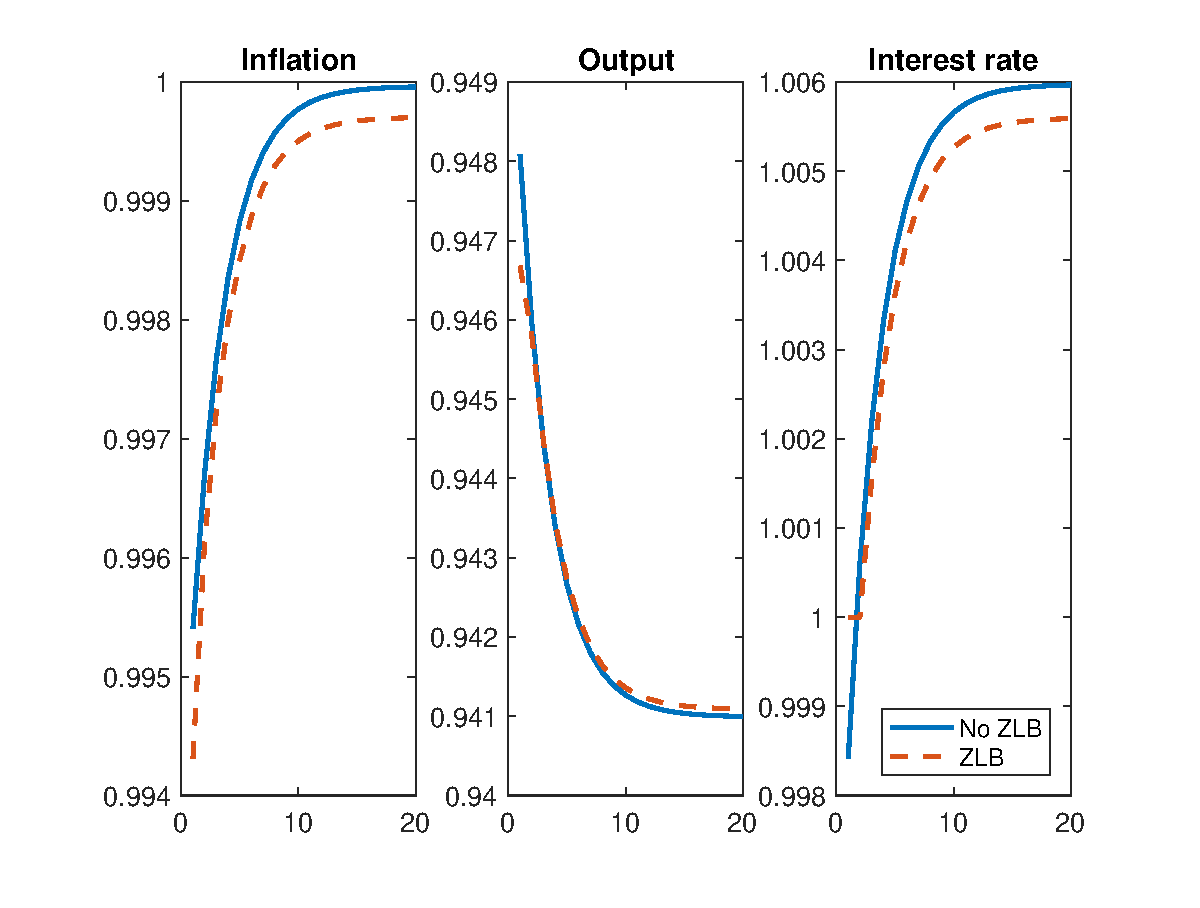
\includegraphics[scale=.6]{m1_irfLevel}
%\end{figure}
%
%\begin{figure}[H]
%	\centering
%	\caption{IFRs--Variables in expectation}\label{fig:m1_irfExp}
%	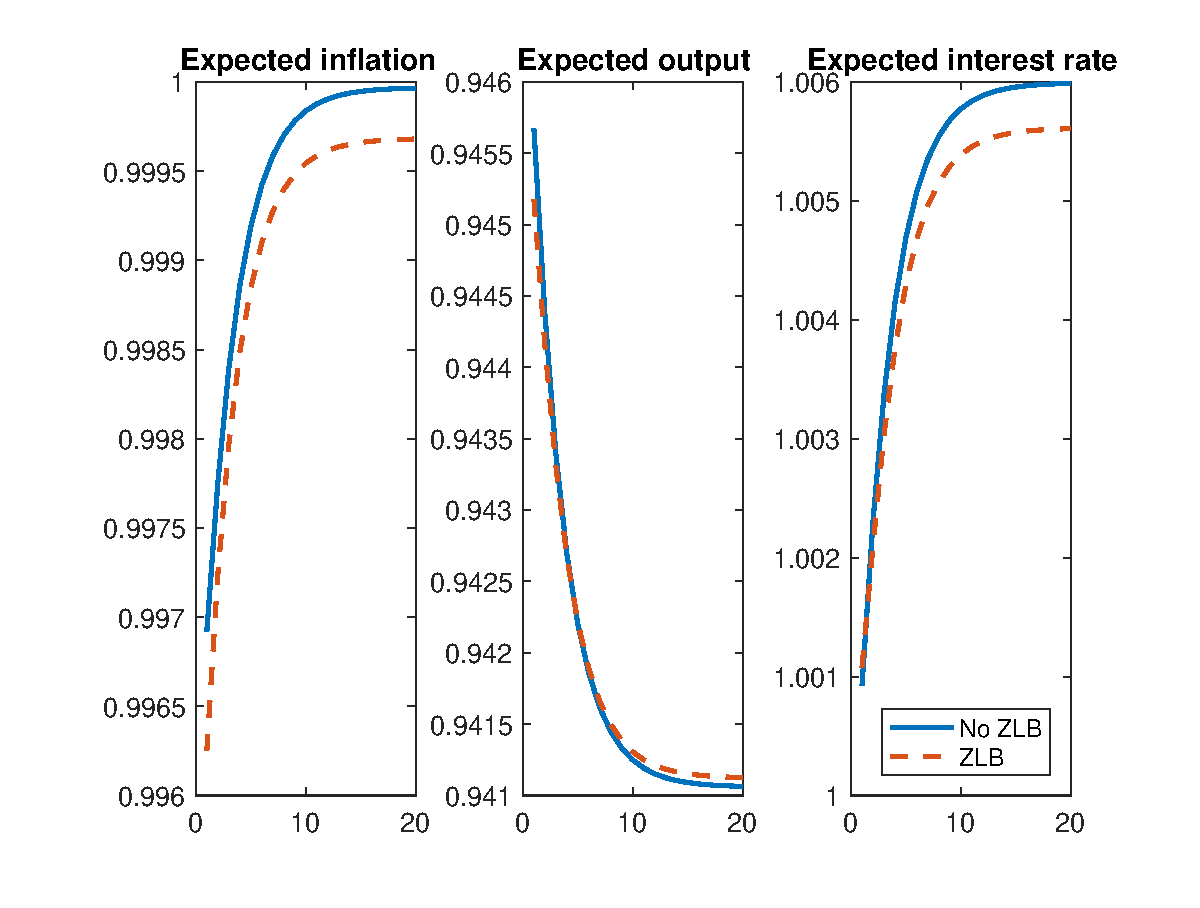
\includegraphics[scale=.6]{m1_irfExp}
%\end{figure}
%
%This exercise shows the long-run distribution of selected variables from a 100,000 simulation of periods.
%
%\begin{figure}[H]
%	\centering
%	\caption{Distribution--Variables in levels (probability)}\label{fig:m1_DistLevel}
%	\includegraphics[scale=.6]{m1_DistLevel}
%\end{figure}
%
%\begin{figure}[H]
%	\centering
%	\caption{Distribution--Variables in expectation (probability)}\label{fig:m1_DistExp}
%	\includegraphics[scale=.6]{m1_DistExp}
%\end{figure}

\section{TFP + preferences shock + output gap}

This version considers TFP and preferences shocks. Also, we consider output gap (the difference between output and natural output) as the relevant measure of activity for monetary authority.

\subsection{Equations of the model}

\begin{align}
	\frac{W_t}{P_t}&=C_t^{\sigma}N_t^{\varphi}\label{app:m2_intra}\\
	1&=R_t\mathbb{E}_t\left\{\beta_{t+1}\left(\frac{C_t}{C_{t+1}}\right)^{\sigma}\frac{1}{\Pi_{t+1}}\right\}\label{app:m2_euler}\\
	(1-\varepsilon)+\varepsilon RMC_t-\zeta(\Pi_t-1)\Pi_t&=-\mathbb{E}_t\left\{\beta_{t+1}\left(\frac{C_t}{C_{t+1}}\right)^{\sigma}\zeta(\Pi_{t+1}-1)\Pi_{t+1}\frac{Y_{t+1}}{Y_t}\right\}\label{app:m2_pricing}\\
	RMC_t&=\frac{W_t}{A_tP_t}\label{app:m2_rmc}\\
	\frac{R_t}{\overline R}&=\max\left\{\left(\frac{\Pi_t}{\overline\Pi}\right)^{\phi_{\pi}}\left(\frac{Y_t^g}{\overline{Y^g}}\right)^{\phi_{y}},1\right\}\label{app:m2_taylor}\\
	Y_t&=A_tN_t\label{app:m2_product}\\
	Y_t&=\left[\frac{1}{1-(\zeta/2)(\Pi_t-1)^2}\right]C_t\label{app:m2_aggregate}\\
	\log A_t&=\rho_a\log A_{t-1}+\sigma_a\epsilon_t^A\label{app:m2_ar1_a}\\
	\log \beta_t&=(1-\rho_{\beta})\log\overline\beta+\rho_{\beta}\log \beta_{t-1}+\sigma_{\beta}\epsilon_t^{\beta}\label{app:m2_ar1_b}\\
	Y_t^g&=\frac{Y_t}{Y_t^n}\label{app:m2_og}
\end{align}
	
We need to derive also the natural level of output. For this, we assume the economy faces no cost to change prices. This is, $\zeta=0$. With this assumption, from \eqref{app:m2_pricing} we have

\begin{align*}
	RMC_t&=\frac{\varepsilon-1}{\varepsilon}\\
	\frac{W_t}{P_t}&=A_tRMC_t
\end{align*}

Also we have $Y_t^n=C_t=A_tN_t$. Replacing in \eqref{app:m2_intra}

\begin{align}
	\frac{W_t}{P_t}&=(Y_t^n)^{\sigma}\left(\frac{Y_t^n}{A_t}\right)^{\varphi}\nonumber\\
	Y_t^n&=A_t^{\frac{\varphi}{\sigma+\varphi}}\left(\frac{W_t}{P_t}\right)^{\frac{1}{\sigma+\varphi}}\label{app:m2_yn}
\end{align}

\subsection{Steady state}

The steady state of inflation equals the level targeted by the authority, which is a zero steady state inflation

\begin{align*}
	\Pi=\overline\Pi=1
\end{align*}

From the Euler equation

\begin{align*}
	R=\frac{\Pi}{\beta}
\end{align*}

From \eqref{app:m2_pricing}

\begin{align*}
	RMC=\frac{\varepsilon-1}{\varepsilon}=\frac{W}{P}
\end{align*}

On the other hand we have

\begin{align*}
	Y=C=N
\end{align*}

Replacing in \eqref{app:m2_intra}

\begin{align*}
	\frac{W}{P}&=C^{\sigma+\varphi}\\
	C&=\left(\frac{W}{P}\right)^{\frac{1}{\sigma+\varphi}}
\end{align*}

And with this we recover $Y$ and $N$. Finally $Y^n=(W/P)^{\frac{1}{\sigma+\varphi}}$.\\

In general, many papers have noticed that these kinds of models have multiple steady states: at least one with a positive nominal interest rate and zero inflation and one with zero interest rate and negative inflation.\footnote{See for example \cite{BenhabibEtAl2001}, \cite{BenhabibEtAl2001a}, \cite{BenhabibEtAl2002} and \cite{Fernandez-VillaverdeEtAl2015}, among others.} However, in this particular formulation of the model, we just have one steady state, characterized by a positive level for the interest rate and a zero steady state inflation. This is due to the calibration of the model, in which utility function shows risk aversion $\sigma\geq1$, so the output gap is not zero in the long run.

\subsection{Calibration}

To calibrate the model we follow \cite{Fernandez-VillaverdeEtAl2015} in most of the parameters. The exception is given for the elasticity of substitution where we set $\sigma=2$. 

In this case, where we have output gap as the relevant activity measure considered by the monetary authority, we set steady state inflation equal to one, which is the only level consistent with the equilibrium of the model. The value in table is used for the solution of the model considering variations of output with respect to the equilibrium level as the activity measure in the Taylor rule, which is the second way we have to solve the problem.

% Table generated by Excel2LaTeX from sheet 'Calibration'
\begin{table}[H]
  \centering
  \caption{Calibration}
    \begin{tabular}{lcc}
    \toprule
    Parameter & Symbol & Value \\
    \midrule
    Steady-state discount factor & $\overline{\beta}$ & 0.994 \\
    Elasticity of substitution & $1/\sigma$ & 1/2 \\
    Frisch elasticity & $1/\varphi$ & 1 \\
    Elasticity of substitution between goods & $\varepsilon$ & 6 \\
    Frequency of price adjustment in Calvo & $\theta$ & 0.75 \\
    Rotemberg adjustment cost & $\zeta=\frac{(\varepsilon-1)\theta}{(1-\theta)(1-\overline{\beta}\theta)}$ & 58.9391 \\
    Monetary policy response to inflation & $\phi_{\pi}$ & 1.5 \\
    Monetary policy response to activity & $\phi_y$ & 0.25 \\
    Steady-state inflation  & $\overline{\Pi}$ & 1.005 \\
    Steady-state output & $\overline{Y}$ & 0.9416 \\
    Steady-state interest rate & $\overline{R}=\frac{\overline{\Pi}}{\overline{\beta}}$ & 1.0111 \\
%    TFP persistence & $\rho_a$ & 0.7 \\
%    TFP volatility & $\sigma_a$ & 0.007 \\
    Discount factor persistence & $\rho_b$ & 0.8 \\
    Discount factor volatility & $\sigma_b$ & 0.0025 \\    
    \bottomrule
    \end{tabular}%
  \label{tab:calibration}%
\end{table}%

\subsection{Solution method}

We solve the model using collocation and different basis functions. The best solution, in terms of computational time and accuracy of the solution, is given by a Chebyshev polynomial approach. We verify that the the policy function for interest rate was not very different to the policy obtained by linear splines, which should be the baseline alternative to solve these kinds of problems. In the end, we solve the model considering a linearly spaced grid that covers four standard deviations for TFP and discount factor respectively.

\subsection{Results}

\paragraph{Approximation errors} In Table \ref{tab:m2_apperror} we present the Euler residual equations and the consumption error, derived from the same equation, using a grid of 100 points for each shock. As we can see, the approximation errors in the solution of the model are less than a 0.2\%.

The formula used to compute the consumption error ($\delta$) comes from the consumption Euler equation

\begin{align*}
	[C_t(1-\delta)]^{-\sigma}&=R_t\mathbb{E}_t\left\{\beta_{t+1}\left(\frac{1}{C_{t+1}}\right)^{\sigma}\frac{1}{\Pi_{t+1}}\right\}\\
	\delta&=1-\frac{\left[R_t\mathbb{E}_t\left\{\beta_{t+1}\left(\frac{1}{C_{t+1}}\right)^{\sigma}\frac{1}{\Pi_{t+1}}\right\}\right]^{-1/\sigma}}{C_t}
\end{align*}

% Table generated by Excel2LaTeX from sheet 'Residual errors'
\begin{table}[H]
  \centering
  \caption{Approximation errors ($\times100$)}
  \resizebox{\textwidth}{!}{
    \begin{tabular}{lcccc}
    \toprule
          & Mean Euler residual & Max Abs Euler residual & Mean consumption error & Max Abs consumption error \\
    \midrule
    Without ZLB & \multicolumn{1}{c}{0.001} & \multicolumn{1}{c}{0.097} & \multicolumn{1}{c}{0.000} & \multicolumn{1}{c}{0.004} \\
    With ZLB & \multicolumn{1}{c}{0.001} & \multicolumn{1}{c}{0.196} & \multicolumn{1}{c}{0.001} & \multicolumn{1}{c}{0.064} \\
    \bottomrule
    \end{tabular}}
  \label{tab:m2_apperror}%
\end{table}%

\paragraph{Impulse-response functions} In this exercise we show the impulse-response function to a one standard deviation shock in the relevant variables. First, we show a positive technology shock, leaving constant the discount factor in its long-run value. We show results in Figures \ref{fig:m2_irfLevel_tfp} and \ref{fig:m2_irfExp_tfp}

\begin{figure}[H]
	\centering
	\caption{Response of variables in levels to a technology shock}\label{fig:m2_irfLevel_tfp}
	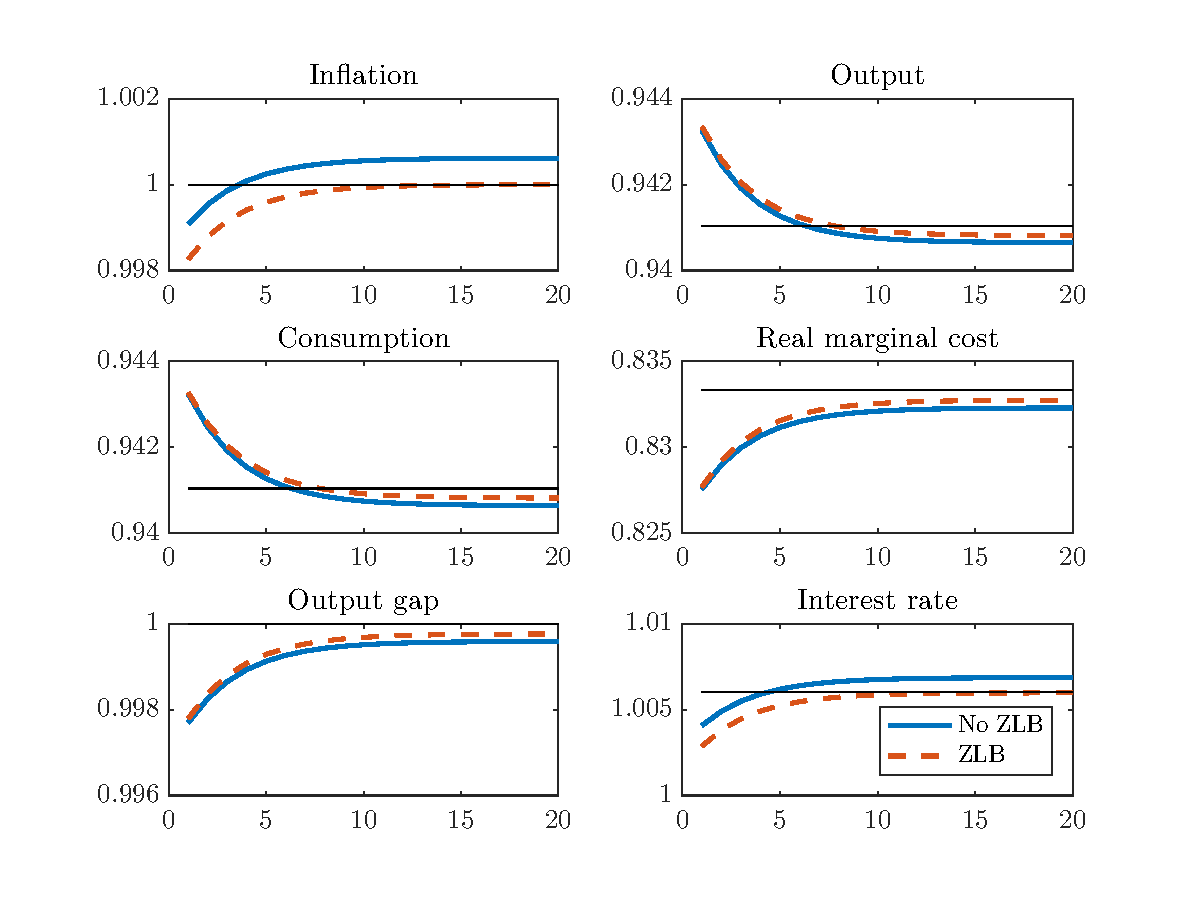
\includegraphics[scale=0.7]{m2_irfLevel_tfp}
\end{figure}

\begin{figure}[H]
	\centering
	\caption{Response of variables in expectation to a technology shock}\label{fig:m2_irfExp_tfp}
	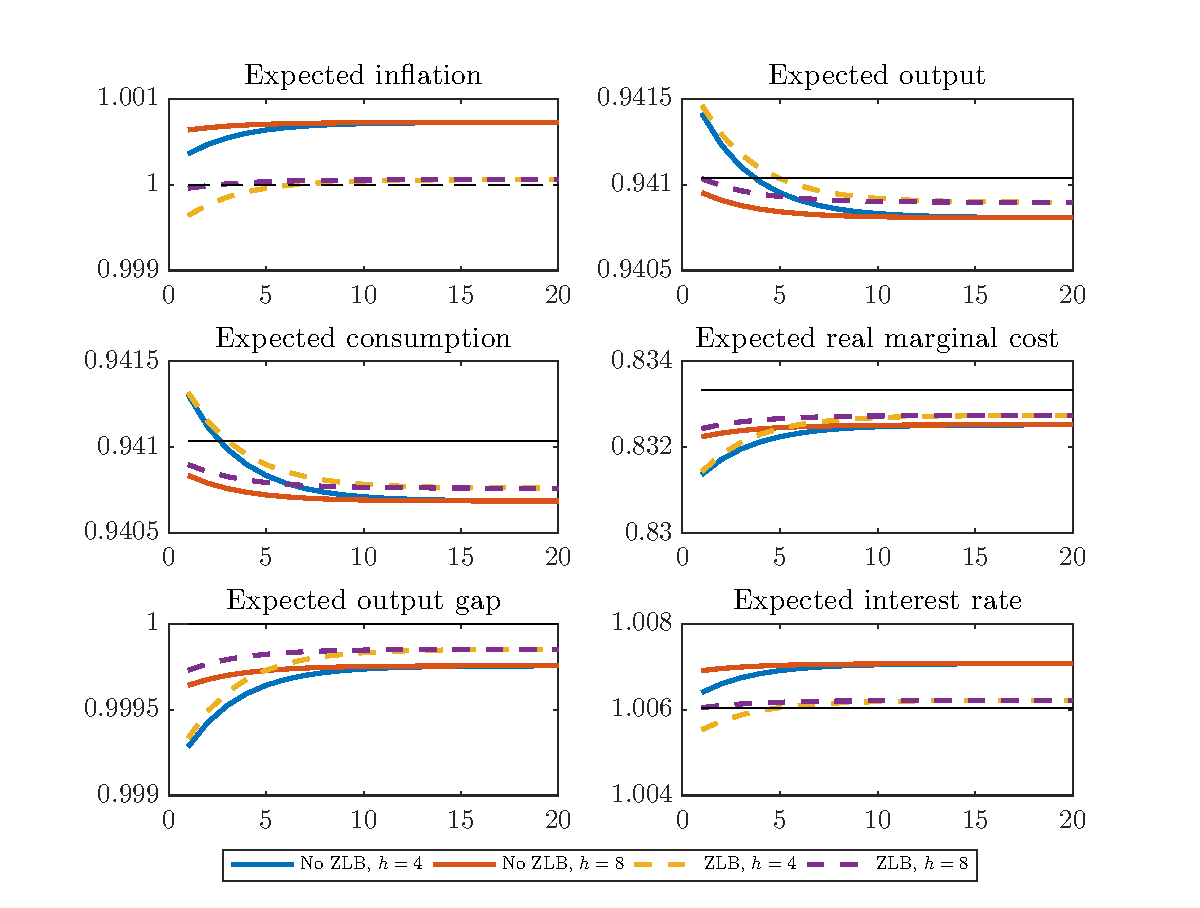
\includegraphics[scale=0.7]{m2_irfExp_tfp}
\end{figure}

\begin{figure}[H]
	\centering
	\caption{Response of variables in levels to a demand shock}\label{fig:m2_irfLevel_pref}
	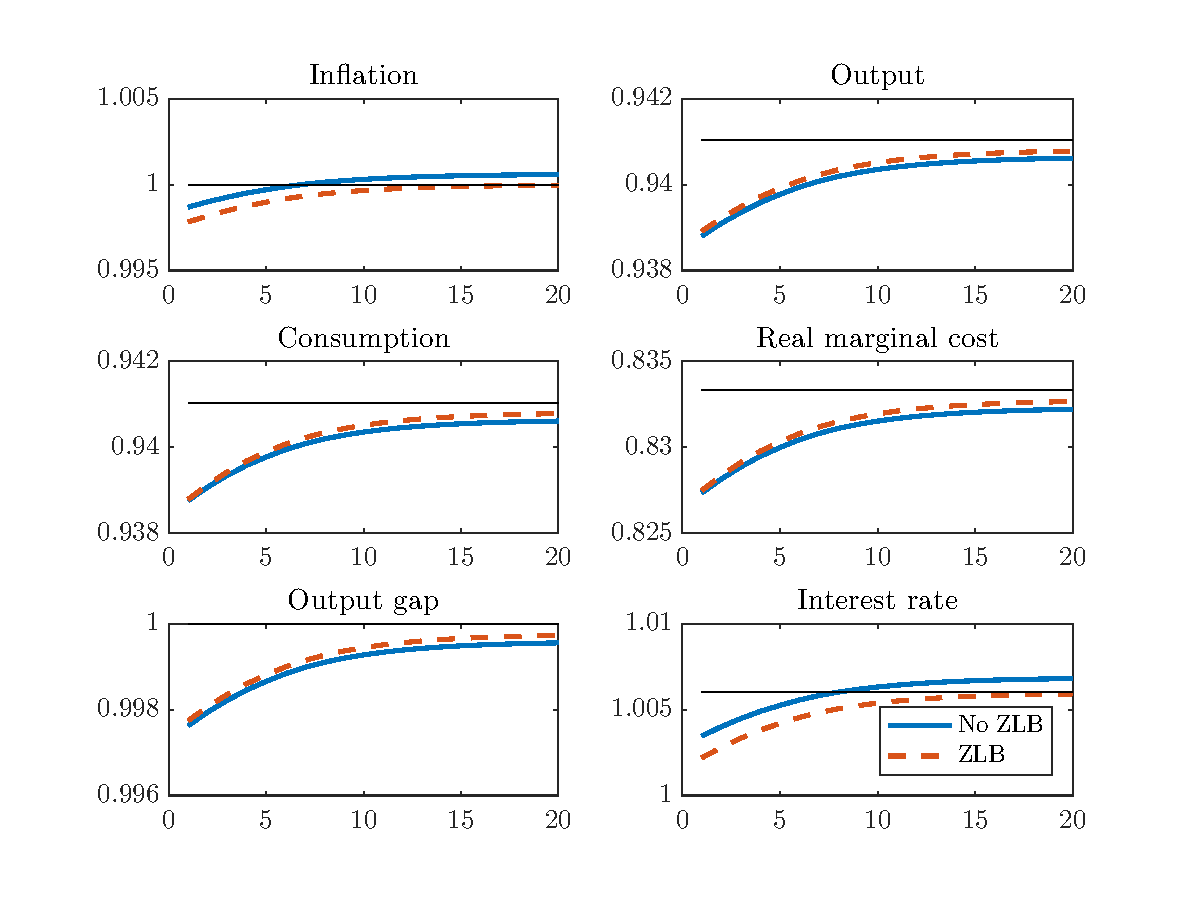
\includegraphics[scale=0.7]{m2_irfLevel_pref}
\end{figure}

\begin{figure}[H]
	\centering
	\caption{Response of variables in expectation to a demand shock}\label{fig:m2_irfExp_pref}
	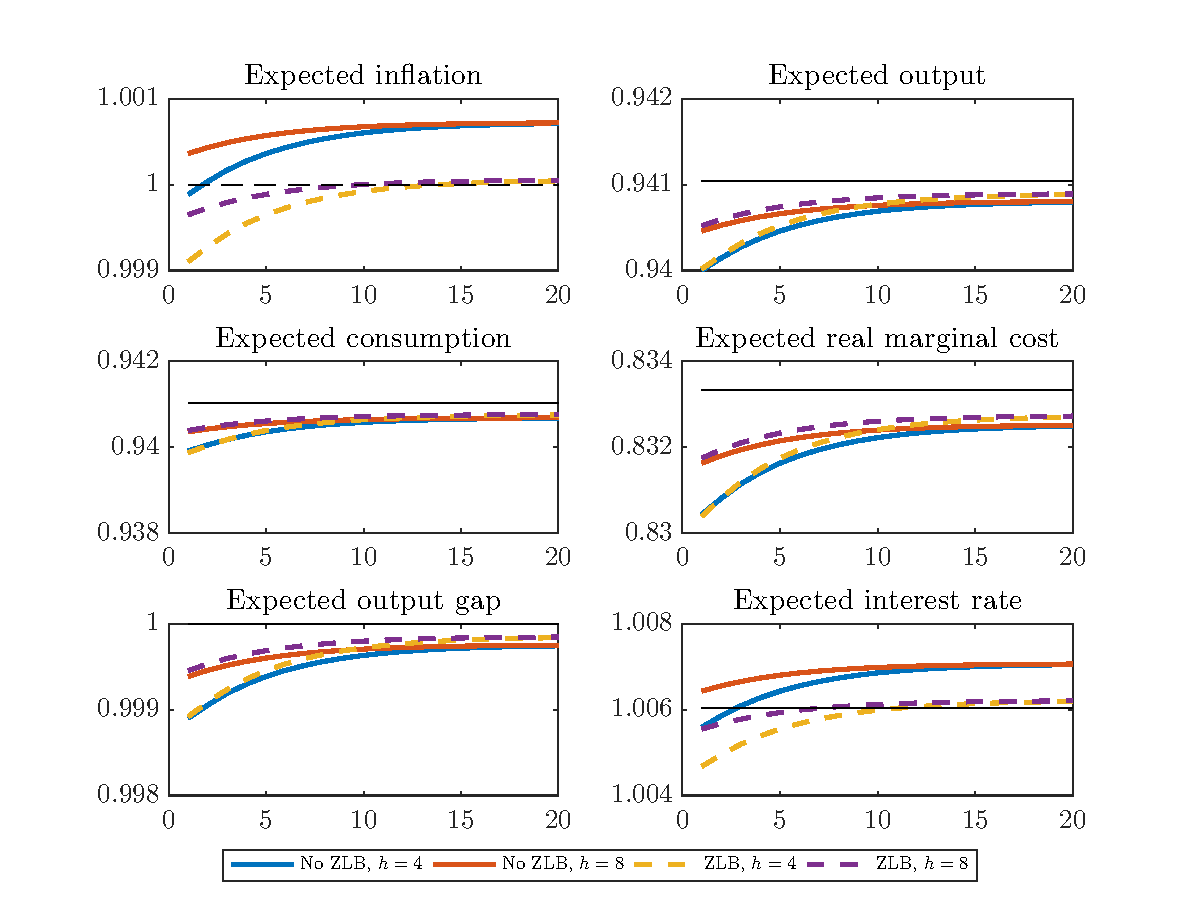
\includegraphics[scale=0.7]{m2_irfExp_pref}
\end{figure}

\paragraph{Ergodic distribution} In Figures \ref{fig:m2_distLevel} and \ref{fig:m2_distExp} we plot the ergodic distribution of selected variables of the model, both in levels and in expectations.

\begin{figure}[H]
	\centering
	\caption{Ergodic distribution of variables in levels}\label{fig:m2_distLevel}
	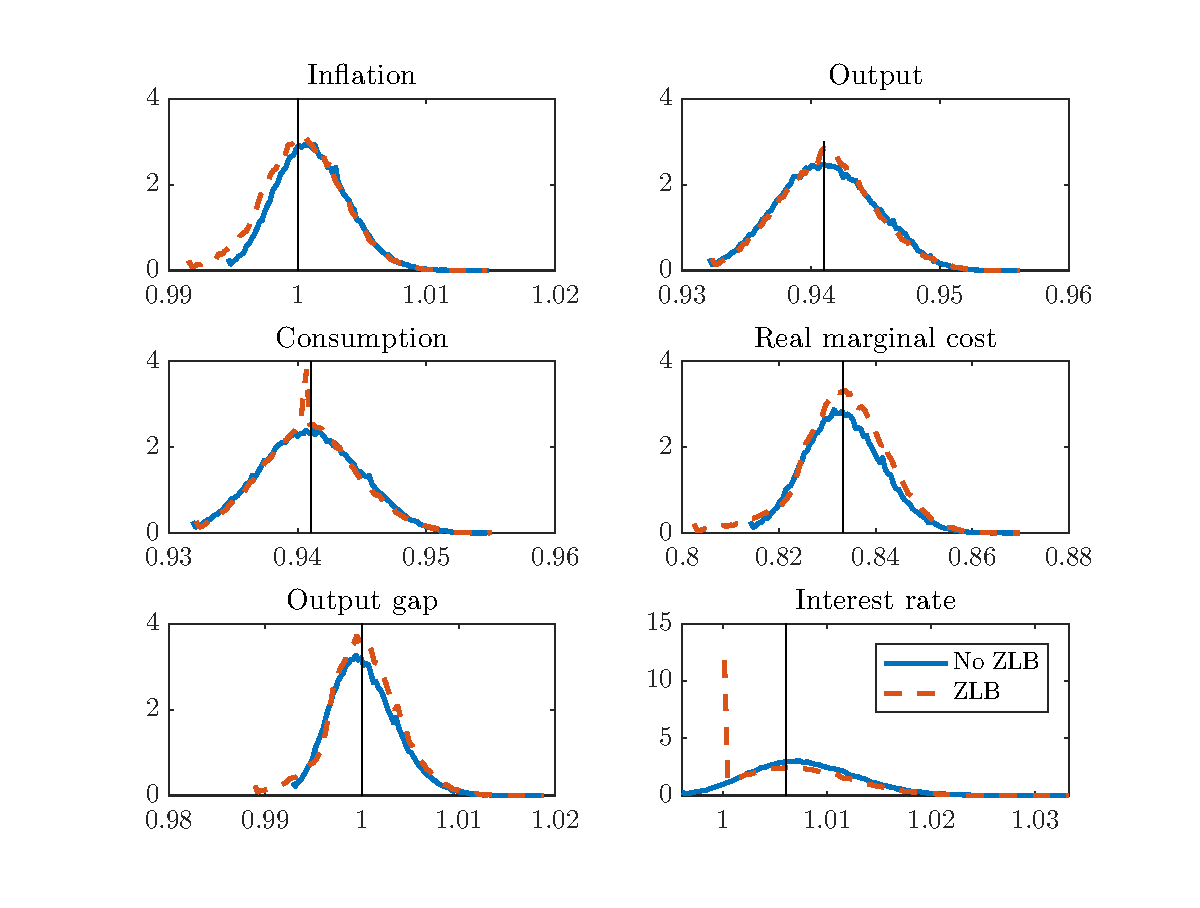
\includegraphics[scale=0.7]{m2_distLevel}
\end{figure}

\begin{figure}[H]
	\centering
	\caption{Ergodic distribution of variables in levels}\label{fig:m2_distExp}
	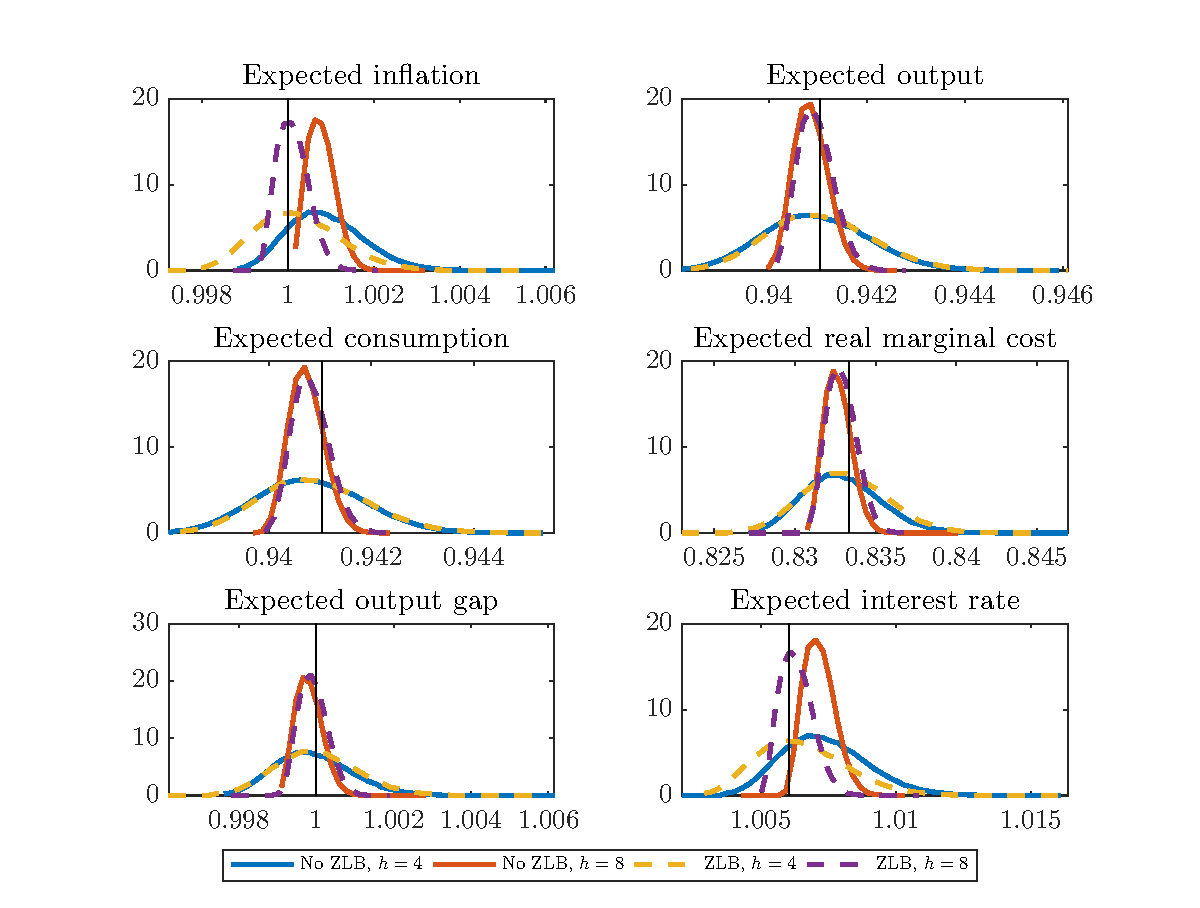
\includegraphics[scale=0.7]{m2_distExp}
\end{figure}

\section{TFP + preferences shock + output deviations from target}

\subsection{Equations of the model}

The main difference with respect to the model presented in previous section is in the Taylor rule, which is now written as

\begin{align*}
	\frac{R_t}{\overline R}&=\left(\frac{\Pi_t}{\overline\Pi}\right)^{\phi_{\pi}}\left(\frac{Y_t}{\overline{Y}}\right)^{\phi_{y}}\label{app:m3_taylor}
\end{align*}

Now, the relevant activity measure for monetary authority is the deviation of output with respect to the target level and not the output gap. This allows us to have two variables and two equations less to track (natural output and output gap).

\subsection{Steady state}

The functional form of the steady state is exactly as before. The exception now is that we can choose different combinations of inflation and interest rate and not just one as before (zero inflation rate and a positive interest rate).

\subsection{Calibration}

The calibration presented in Table \ref{tab:calibration} applies.

\subsection{Solution method}

The same solution method of the previous model applies.

\subsection{Results}

\paragraph{Approximation errors} As in the previous model, we compute approximation errors of our solution method, which are presented in Table \ref{tab:m3_apperror}. As we can see, the errors are of the same magnitude as before (slightly smaller).

% Table generated by Excel2LaTeX from sheet 'Residual errors'
\begin{table}[H]
  \centering
  \caption{Approximation errors ($\times100$)}
  \resizebox{\textwidth}{!}{
    \begin{tabular}{lcccc}
    \toprule
          & Mean Euler residual & Max Abs Euler residual & Mean consumption error & Max Abs consumption error \\
    \midrule
    Without ZLB & \multicolumn{1}{c}{0.000} & \multicolumn{1}{c}{0.116} & \multicolumn{1}{c}{0.000} & \multicolumn{1}{c}{0.005} \\
    With ZLB & \multicolumn{1}{c}{0.000} & \multicolumn{1}{c}{0.157} & \multicolumn{1}{c}{0.000} & \multicolumn{1}{c}{0.047} \\
    \bottomrule
    \end{tabular}}
  \label{tab:m3_apperror}%
\end{table}%

\paragraph{Impulse-response functions} 

\begin{figure}[H]
	\centering
	\caption{Response of variables in levels to a technology shock}\label{fig:m2_irfLevel_tfp}
	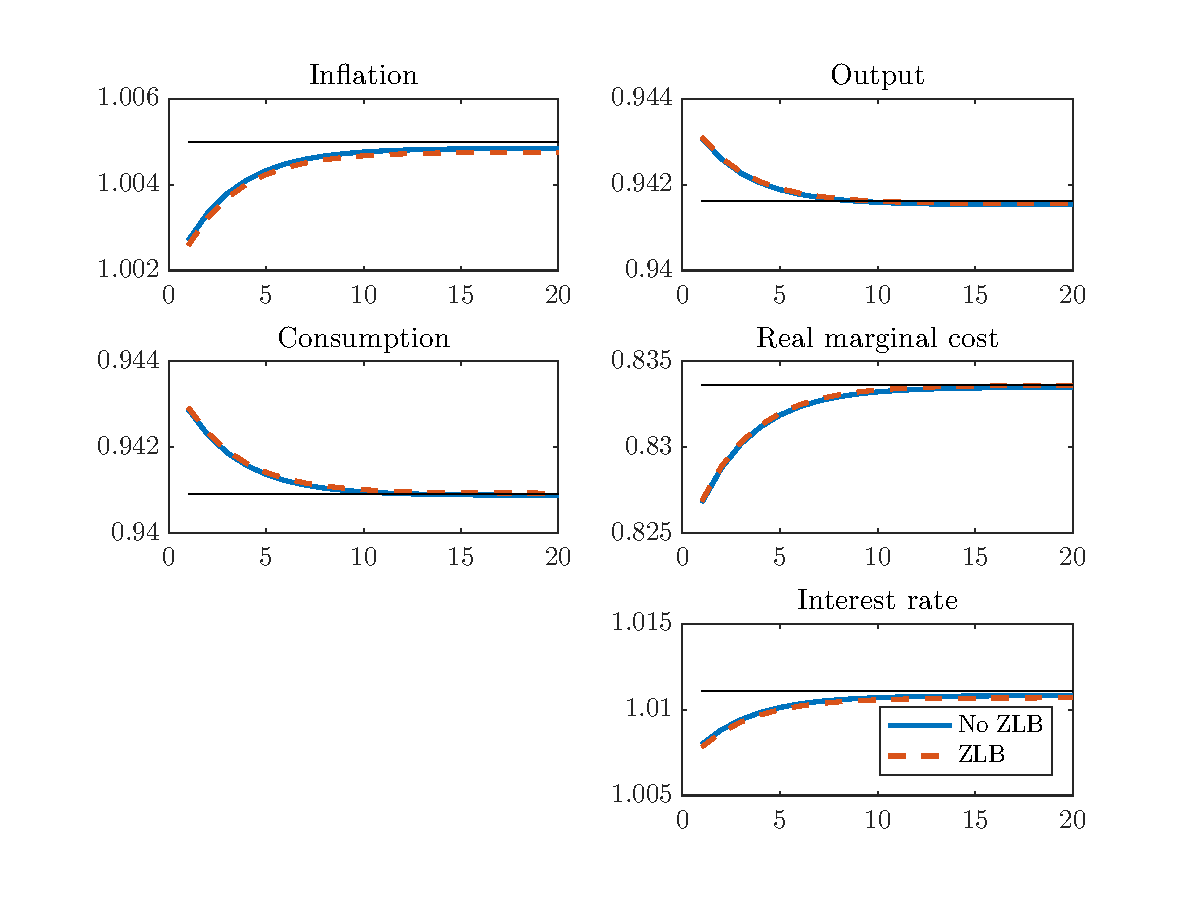
\includegraphics[scale=0.7]{m3_irfLevel_tfp}
\end{figure}

\begin{figure}[H]
	\centering
	\caption{Response of variables in expectation to a technology shock}\label{fig:m2_irfExp_tfp}
	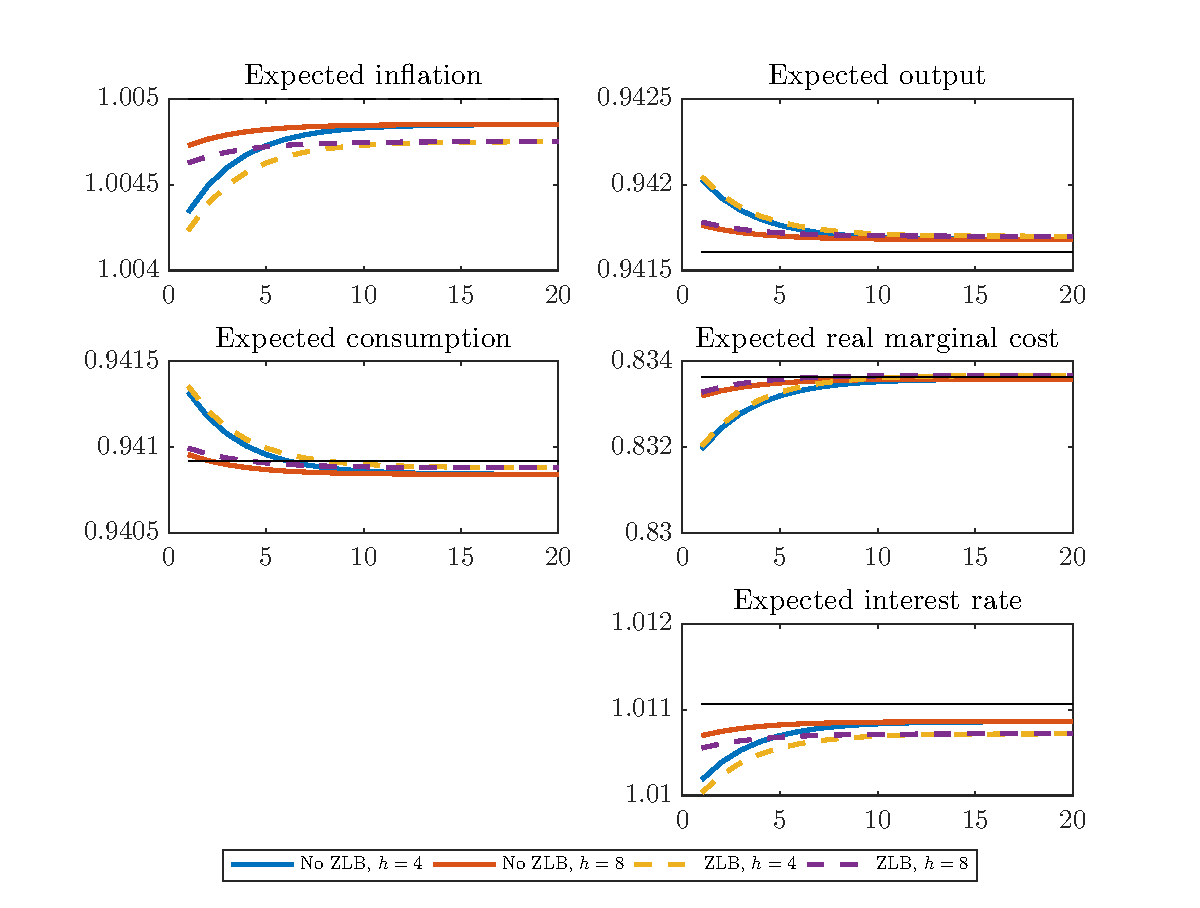
\includegraphics[scale=0.7]{m3_irfExp_tfp}
\end{figure}

\begin{figure}[H]
	\centering
	\caption{Response of variables in levels to a demand shock}\label{fig:m2_irfLevel_pref}
	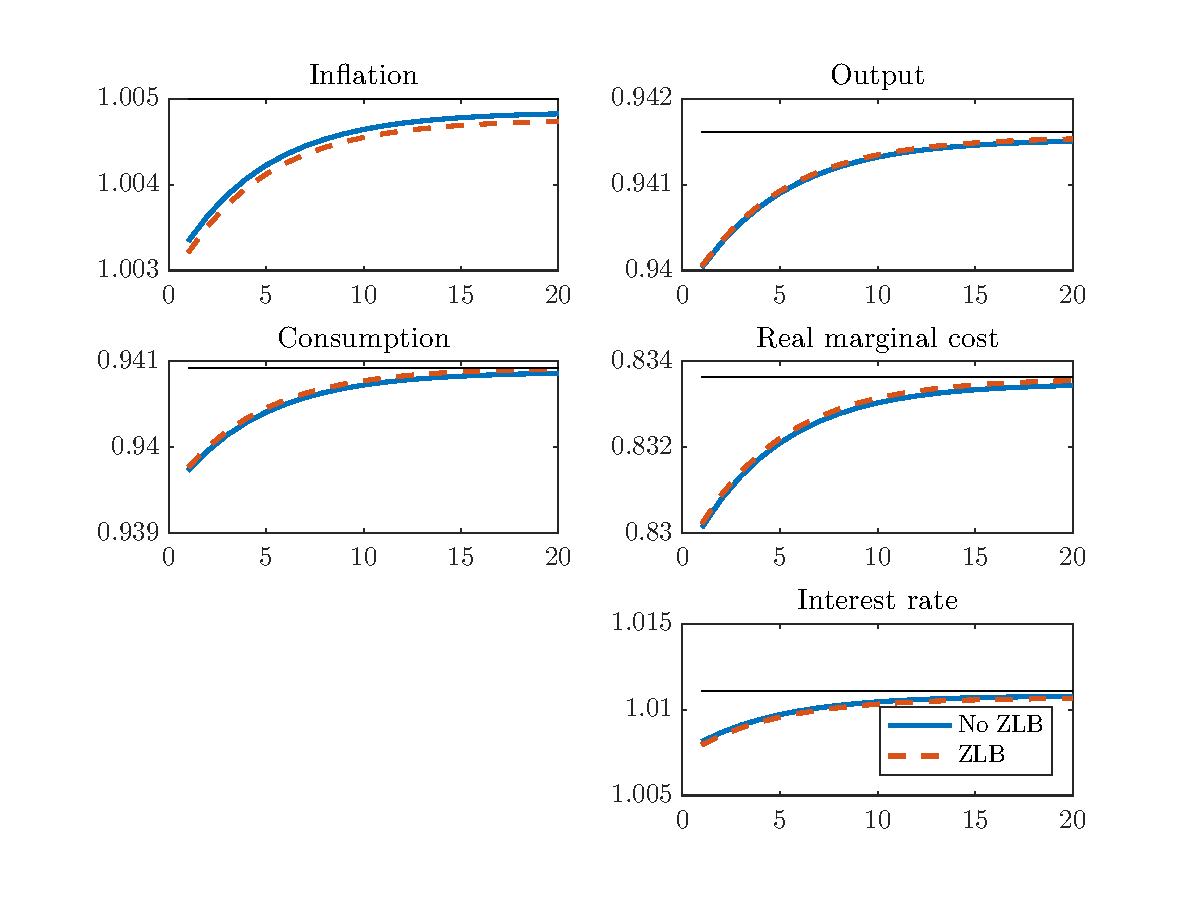
\includegraphics[scale=0.7]{m3_irfLevel_pref}
\end{figure}

\begin{figure}[H]
	\centering
	\caption{Response of variables in expectation to a demand shock}\label{fig:m2_irfExp_pref}
	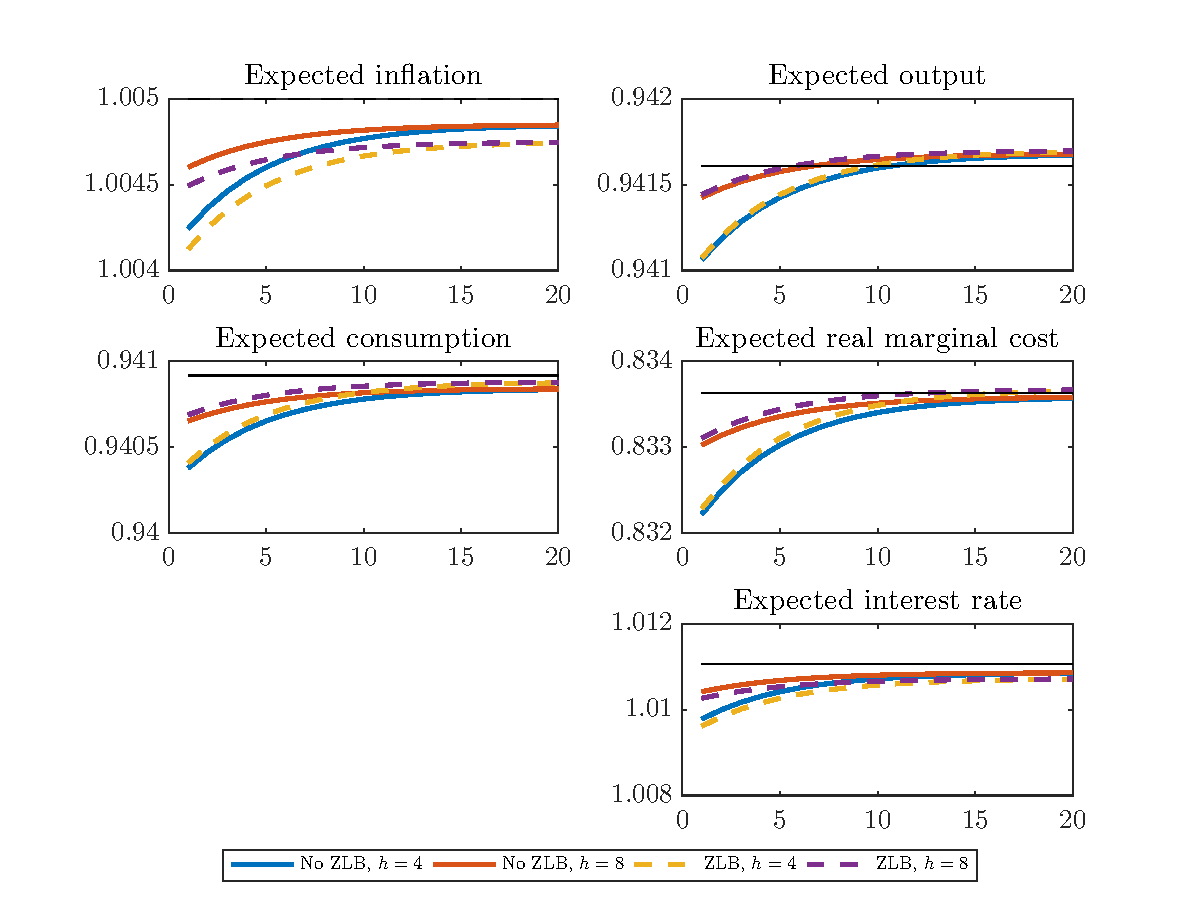
\includegraphics[scale=0.7]{m3_irfExp_pref}
\end{figure}

\paragraph{Ergodic distribution}

\begin{figure}[H]
	\centering
	\caption{Ergodic distribution of variables in levels}\label{fig:m3_distLevel}
	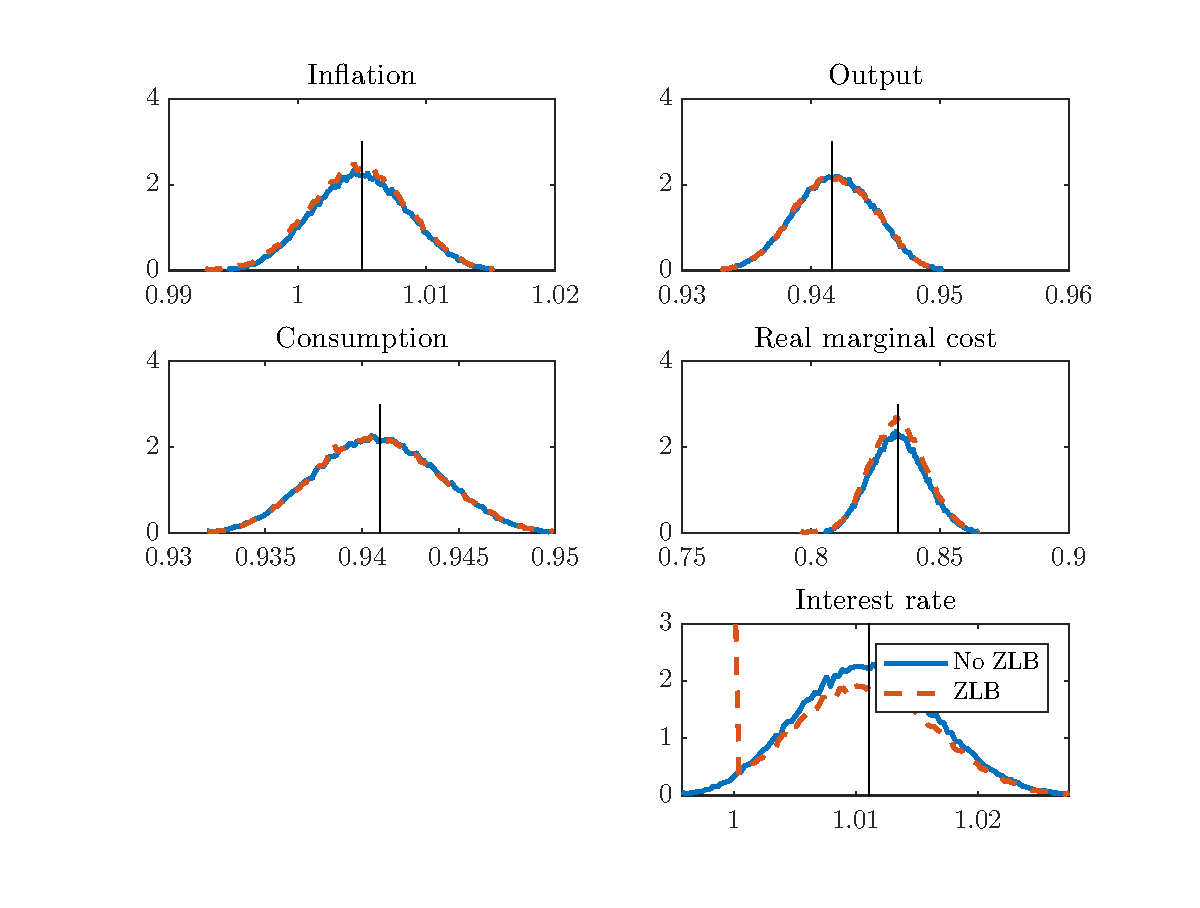
\includegraphics[scale=0.7]{m3_distLevel}
\end{figure}

\begin{figure}[H]
	\centering
	\caption{Ergodic distribution of variables in levels}\label{fig:m3_distExp}
	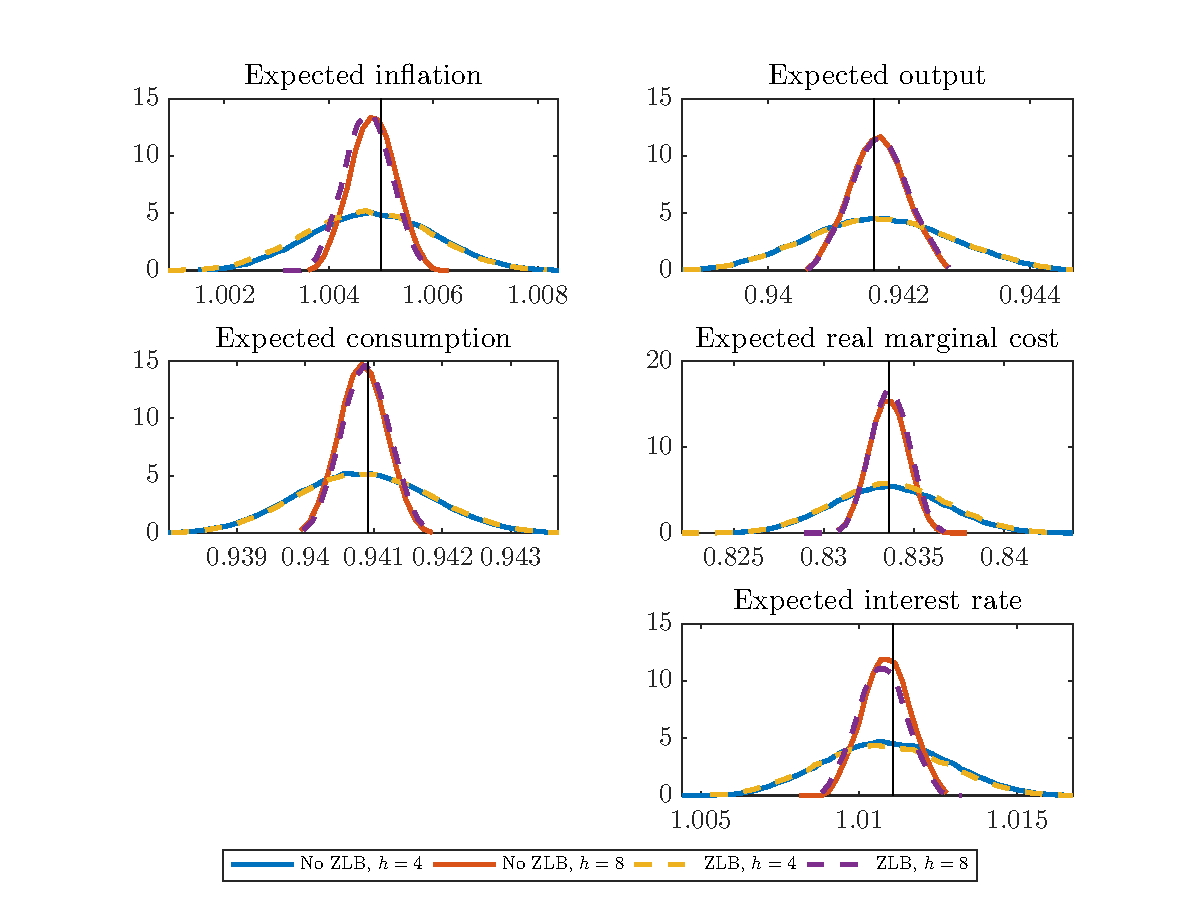
\includegraphics[scale=0.7]{m3_distExp}
\end{figure}

%%GATHER{tbib.bib}
\bibliographystyle{agsm}
\bibliography{tbib}
	
\end{document}
